\documentclass[12pt,]{article}
\usepackage{lmodern}
\usepackage{amssymb,amsmath}
\usepackage{ifxetex,ifluatex}
\usepackage{fixltx2e} % provides \textsubscript
\ifnum 0\ifxetex 1\fi\ifluatex 1\fi=0 % if pdftex
  \usepackage[T1]{fontenc}
  \usepackage[utf8]{inputenc}
\else % if luatex or xelatex
  \ifxetex
    \usepackage{mathspec}
    \usepackage{xltxtra,xunicode}
  \else
    \usepackage{fontspec}
  \fi
  \defaultfontfeatures{Mapping=tex-text,Scale=MatchLowercase}
  \newcommand{\euro}{€}
\fi
% use upquote if available, for straight quotes in verbatim environments
\IfFileExists{upquote.sty}{\usepackage{upquote}}{}
% use microtype if available
\IfFileExists{microtype.sty}{%
\usepackage{microtype}
\UseMicrotypeSet[protrusion]{basicmath} % disable protrusion for tt fonts
}{}
\usepackage[margin=1in]{geometry}
\usepackage{natbib}
\bibliographystyle{plainnat}
\usepackage{longtable,booktabs}
\usepackage{graphicx}
\makeatletter
\def\maxwidth{\ifdim\Gin@nat@width>\linewidth\linewidth\else\Gin@nat@width\fi}
\def\maxheight{\ifdim\Gin@nat@height>\textheight\textheight\else\Gin@nat@height\fi}
\makeatother
% Scale images if necessary, so that they will not overflow the page
% margins by default, and it is still possible to overwrite the defaults
% using explicit options in \includegraphics[width, height, ...]{}
\setkeys{Gin}{width=\maxwidth,height=\maxheight,keepaspectratio}
\ifxetex
  \usepackage[setpagesize=false, % page size defined by xetex
              unicode=false, % unicode breaks when used with xetex
              xetex]{hyperref}
\else
  \usepackage[unicode=true]{hyperref}
\fi
\hypersetup{breaklinks=true,
            bookmarks=true,
            pdfauthor={Michael C Sachs and Lisa M McShane},
            pdftitle={Issues in developing multivariable models for treatment selection},
            colorlinks=true,
            citecolor=blue,
            urlcolor=blue,
            linkcolor=magenta,
            pdfborder={0 0 0}}
\urlstyle{same}  % don't use monospace font for urls
\setlength{\parindent}{0pt}
\setlength{\parskip}{6pt plus 2pt minus 1pt}
\setlength{\emergencystretch}{3em}  % prevent overfull lines
\setcounter{secnumdepth}{0}

%%% Use protect on footnotes to avoid problems with footnotes in titles
\let\rmarkdownfootnote\footnote%
\def\footnote{\protect\rmarkdownfootnote}

%%% Change title format to be more compact
\usepackage{titling}

% Create subtitle command for use in maketitle
\newcommand{\subtitle}[1]{
  \posttitle{
    \begin{center}\large#1\end{center}
    }
}

\setlength{\droptitle}{-2em}
  \title{Issues in developing multivariable models for treatment selection}
  \pretitle{\vspace{\droptitle}\centering\huge}
  \posttitle{\par}
  \author{Michael C Sachs and Lisa M McShane}
  \preauthor{\centering\large\emph}
  \postauthor{\par}
  \predate{\centering\large\emph}
  \postdate{\par}
  \date{May 10, 2016}



\begin{document}

\maketitle


\section{Abstract}\label{abstract}

Omics technologies that generate a large amount of molecular data about
biospecimens have the potential to provide information about a patient's
disease characteristics above and beyond standard clinical and
pathological features. By combining the information from a large amount
of molecular features into a multivariable model, called a biomarker
signature, there is the opportunity to identify distinct subgroups of
patients for whom treatment decisions can be personalized. A biomarker
signature can guide the decisions to treat or not to treat and help
identify the patients who are most likely to survive. The key challenge
is to combine features from a high dimensional molecular assay to derive
a signature with good clinical performance and appropriately
characterize its performance. The inappropriate practice of using
overlapping data to both build a signature and evaluate its performance
can lead to severe over-optimism bias in performance estimates. We
summarize the key statistical issues and methods for developing and
validating biomarker signatures, using examples from the literature to
illustrate them.

\section{Introduction}\label{introduction}

Omics technologies that generate a large amount of molecular data about
biospecimens have the potential to provide information about a patient's
disease characteristics above and beyond standard clinical and
pathological features. By combining the information from a large amount
of molecular features into a multivariable model, hereafter referred to
as a \emph{biomarker signature}, there is the opportunity to identify
distinct subgroups of patients for whom treatment decisions can be
personalized. A multivariable biomarker can guide the decisions to treat
or not to treat and help identify the patients who are most likely to
survive. The key challenge we address in this paper is how to combine
features from a high dimensional molecular assay to derive a signature
that is fit for a specified clinical use and to provide valid estimates
of performance characteristics.

\subsection{Terminology and Notation}\label{terminology-and-notation}

A \textbf{biomarker signature} is a transformation of multiple
individual features, typically molecular characterstics measured on a
multiplex assay, to a one-dimensional space. Specifically, let \(X\)
denote the set of \(p\) features under consideration. The signature is
an unknown function \(f(X): \mathbb{R}^p \mapsto \mathbb{R}^1\). The
signature result may be continuous, take multiple discrete values, or be
dichotomous.

Let \(S\) denote the development dataset which includes, for each of
\(n\) represented individuals, a feature vector \(X\), an outcome \(Y\),
a treatment \(Z\), and possibly other variables. \(S\) is a sample of
size \(n\) from distribution \(\mathcal{P}\) with domain
\(\mathcal{S}\). Let \(\mathcal{F}\) be a mapping from \(\mathcal{X}\)
to the space of continuous functions with domain \(\mathbb{R}^p\) and
range \(\mathbb{R}\), \(\mathcal{D}\). Thus
\(\mathcal{F}: \mathcal{X} \mapsto \mathcal{D}\) denotes the process or
algorithm through which a particular \(f\) is estimated. We do not place
any other restrictions on \(\mathcal{F}\), it could be a clustering
approach, a regression approach, a combination of both, or something
else entirely. We will use \(\mathcal{F}\) to denote the manner in which
\(f\) is estimated and will write \(f \in \mathcal{F}\) to denote that
\(f\) is estimated with the class of methods \(\mathcal{F}\).

Let \(\phi: \mathcal{D} \times \mathcal{X} \mapsto \mathbb{R}\) denote
the statistic that quantifies the performance of the function \(f\),
such as predictive accuracy, mean squared error, or area under the
receiver operating characteristic (ROC) curve (AUC). This could also be
a measure of association, such as an odds ratio, hazard ratio, or
log-rank statistic. This is a function of both \(f\) and \(S\). We are
interested in estimating \(E_\mathcal{P}[\phi_{f^*}(S)]\), which is the
expected error under the data generation mechanism, for a particular
\(f^* \in \mathcal{F}\). This allows us to understand how the signature
will perform on future observations generated from \(\mathcal{P}\). We
may also be interested in estimating \(E_\mathcal{P}[\phi_f(S)]\)
\emph{for all} \(f \in \mathcal{F}\), which is the generalization error
for \(f\) generated using mechanism \(\mathcal{F}\). This doesn't guide
outside researchers as to which specific \(f\) to use, yet it is useful
for development because it tells us how much signal is in the data. As
shorthand we will write this as \(E_\mathcal{P}[\phi_\mathcal{F}(S)]\)

A signature that \textbf{reliably predicts} an outcome \(Y\) is one that
has generalization error small enough for the clinical context. Such a
signature may be useful for treatment selection, prognosis, or other
type of clinical management.

\subsection{Overview of biomarker signature
development}\label{overview-of-biomarker-signature-development}

The main goal is to produce a good signature. To establish this requires
a valid estimate of the signature's performance. Assessment of the worth
of a biomarker signature requires providing a valid estimate of the
performance of \(f \in \mathcal{F}\). Additionally, one can provide a
specification of \(f\) for others to use. Typically, a specific \(f\) is
estimated using \(\mathcal{F}\) based on some training data. This can be
done using a variety of different methods. In recent years there have
been an explosion in the literature of computational approaches to
classification and prediction, and we do not intend to summarize them
all here. Some excellent reviews of such approaches are
\citet{hastie2009elements} and \citet{moons2012riskI}. The main
considerations in signature estimation are identifying the features to
include, deciding what transformations to apply, determining how to
combine the feature measurements, and whether to apply
thresholds/cutoffs to the resulting signature value.

A biomarker signature can inform clinical practice in a number of ways.
In early-stage disease, a highly prognostic signature may identify a
subpopulation of patients that has such a good chance of long term
survival, that they do not require additional treatment beyond some
standard base therapy. Therefore these good risk patients can be spared
the risks and side-effects associated with additional therapy. In the
context of a specific therapy that targets a particular molecular
pathway, a signature may identify a subpopulation of patients that does
or does not benefit from that therapy, thereby guiding the decision to
treat or not.

Signatures can be estimated by identifying naturally occuring clusters,
or intrinsic subtypes using \(X\) alone without regard to the outcome
\(Y\). The PAM-50 gene signature was developed using clustering methods
in an attempt to identify intrinsic subtypes with different prognosis
\citep{parker2009supervised}. Later, the intrinsic subtypes were shown
to be strongly associated with clinical outcomes
\citep{nielsen2010comparison}. Supervised learning techniques can also
be used to identify prognostic signatures, as was the case with Oncotype
DX \citep{paik2004multigene}, another signature developed for clinical
decision making in early stage breast cancer. In this case,
regression-based methods are used to estimate a model that is highly
predictive for the outcome \(Y\). In the case of Oncotype DX, the
outcome in question was distant recurrence of breast cancer.

An approach to identifying treatment-selection signatures is to use
regression techniques to estimate a signature that has a strong
interaction with a particular treatment. It is possible, and quite
common in high-dimensional settings, to combine multiple approaches to
estimating \(f\). For instance, a data-reduction step by variable
selection or clustering may be performed before doing regression
analysis on the resulting components.

No matter what the particular model building method is, our main concern
and focus of this paper is with obtaining a valid estimate of its
performance, that is, a good estimate of
\(E_\mathcal{P}[\phi_\mathcal{F}(S)]\). This depends on the true signal
in the data and the specific algorithm \(\mathcal{F}\) used. An optional
component of the development phase is to provide a specification of
\(f\) for others to use on independent data or in clinical practice.

\subsection{Biomarker signatures in clinical
practice}\label{biomarker-signatures-in-clinical-practice}

Biomarker signatures are useful if they can correctly and reliably
classify patients into distinct subgroups for which different treatment
decisions would be made. There are two distinct but related statistical
concepts involved here: calibration and discrimination. Signatures are
often optimized to be well-calibrated, that is, accurate for predicting
outcomes. However if the signature does not separate a population into
distinct subgroups with therapeutic relevance, then it is unlikely to be
informative enough to change clinical practice.

In the development process it is important to evaluate both calibration
and discrimination. It is not trivial to assess each of these in a valid
manner when the data are used to define the signature itself. We
illustrate the potential for bias through a series of examples, and we
review some strategies to avoid the pitfalls that lead to bias.

\subsection{Data analysis example}\label{data-analysis-example}

Throughout this paper, we reanalyze data from \citet{zhu2010prognostic}.
Briefly, the data of interest are from the JBR.10 trial, which was a
randomized controlled trial of adjuvant vinorelbine/cisplatin (ACT)
versus observation alone (OBS) in 482 participants with non small cell
lung cancer (NSCLC). Of those 482 participants, 169 had frozen tissue
collected, and of those samples, 133 (71 in ACT and 62 in OBS) had
gene-expression profiling performed using U133A oligonucleotide
microarrays (Affymetrix, Santa Clara, CA).

The goal of the \citet{zhu2010prognostic} paper was to identify a
multi-gene signature that strongly predicts prognosis, and the
hypothesis was that the poor prognosis subgroup would benefit more from
ACT compared to the good prognosis subgroup. The signature was trained
to predict disease specific survival. The annotated gene expression data
and clinical information are available from the Gene Expression Omnibus
(identifier: GSE14814, \citet{edgar2002gene}).

\citet{zhu2010prognostic} present results that mainly focus on the
discrimination ability of their estimated signature. They do that by
demonstrating that the two risk subgroups predicted by their signature
(high risk and low risk) have separation in their survival curves and
that the hazard ratio for their signature is large and significant even
when adjusting for other risk factors. They do not directly address
calibration, that is, whether their signature accurately predicts
survival times.

We used a similar approach to preprocessing as did
\citet{zhu2010prognostic}, as we could not reproduce their workflow
exactly due to outdated software. Batch effects were removed using the
\texttt{ComBat} function in the \texttt{sva} \texttt{R} package
\citep{leeksva} and then the gene expression values were centered by
their means and scaled by their standard deviations. Our signature
development approach is similar but not identical to that in
\citet{zhu2010prognostic}. For purposes of illustrating the concepts we
used a simplyfied approach to signature development that retains the
main features of the original. The exact approach to signature
development does not have a major impact on the main conclusions of our
evaluation of the various approaches to signature performance
assessment.

Following the processing steps described above, we performed a gene
selection step wherein we fit univariate Cox regression models with
disease specific survival as the outcome and each gene as the single
predictor. Genes with univariate p-values less than 0.005 were selected
for further analysis. Then, each gene was weighted by its univariate Cox
regression coefficient, and the resulting weighted gene expression
values summed to form risk scores. Genes were selected in a forward
selection manner, starting with the most significant genes, the gene
that improved the concordance between survival times and the risk score
was selected. If no gene improved the concordance, the process was
stopped. The final list of selected genes were all included in a
multivariable Cox regression model to fit the final risk score. The
cutoff that yielded the smallest log-rank statistic p-value was used to
dichotomize into two risk groups.

\section{Issues}\label{issues}

Recall that the main goal is to estimate
\(E_\mathcal{P}[\phi_\mathcal{F}(S)]\), the expected value of a given
statistic on future observations for \(f \in \mathcal{F}\). This can be
estimated with the in-sample empirical estimate:
\(\hat{E}[\phi_f(S)] = \frac{1}{n}\sum_{i=1}^n\phi_f(s_i)\) for a
particular \(f\). However, if \(S\) is used to estimate \(f\) then the
estimate will be biased due to overfitting, that is,
\(|E_\mathcal{P}[\phi_f(S)] - \hat{E}[\phi_f(S)]|\) will be large. This
bias results from the fact that \(\phi\) depends on \(f\), and thus the
statistic \(\phi\) is being adaptively defined based on the observed
data \(S\). Overfitting occurs when a model is fit to noise in the data.
This often occurs when fitting a model that is overly complex relative
to the amount of signal in the available data.

In many cases during signature development, the performance metric
\(\phi\) in question is a statistic that relates to calibration. While a
biomarker signature may accurately predict a clinical outcome, that does
not neccessarily imply that the signature is clinically useful. To
assess discrimination, a different statistic \(\phi\) may be used, such
as the area under the ROC curve. Measures of association such as the
odds ratio, hazard ratio, or difference in survival probabilities are
examples of performance metrics that are commonly used, although their
value for biomarker signatures has been debated
\citep{pepe2004limitations}. Evaluation of \(\phi\) is subject to bias
due to overfitting regardless of what \(\phi\) is used, a fact that is
commonly overlooked in the medical literature.

In \citet{zhu2010prognostic}, \(\phi\) was the hazard ratio comparing
the high risk and low risk groups as defined by the JBL.10 signature
\(f\). The risk groups were determined by the signature \(f\), which was
estimated using \(S\), the same data that was then used to produce the
hazard ratio estimate of 15. They go on to assess the performance of the
JBL.10 signature in a series of independent data sets, in which they
estimate hazard ratios of approximately 2. Here we reanalyze the dataset
and illustrate some remedies to avoid bias in estimating signature
performance.

\subsection{Avoiding Overfitting}\label{avoiding-overfitting}

A traditional method to avoid overfitting is the split sample approach.
First, randomly partition \(S\) into the training sample \(S_t\) and the
holdout sample \(S_h\) with sample sizes \(n_t\) and \(n_h\),
respectively. Then, \(S_h\) is hidden from the analyst while
\(\mathcal{F}\) is applied to \(S_t\) to estimate the signature function
\(f_t\). For fixed \(f_t\), \(\hat{E}[\phi_{f_t}(S_h)]\) is an unbiased
estimator of both \(E_{\mathcal{P}}[\phi_{f_t}(S)]\) and
\(E_\mathcal{P}[\phi_\mathcal{F}(S)]\). The specific form of \(f_t\)
that is fixed using the \(S_t\) partition can be reported as the
function for others to use, therefore the aforementioned estimator is
also an estimate of the error for that specific \(f_t\). The drawback of
the split-sample approach is that the performance of \(f_t\) is likely
to be inferior to the performance of a function \(f^*\) derived using
the same approach applied to the entire data set.
\citet{dobbin2011optimally} investigate how to optimally split a dataset
into training and holdout partitions.

Another approach to avoid overfitting is cross-validation, which is a
resampling based approach. For a fixed integer \(k\), which can be
between 1 and \(n\), we randomly select a partition of \(k\)
observations from \(S\), denoted \(S_k\). Then \(f_{-k}\) is estimated
and fixed by appling \(\mathcal{F}\) on \(S_{-k}\) which is the subset
of \(S\) that is disjoint from \(S_k\). Then, we get an estimate
\(\hat{E}[\phi_{f_{-k}}(S_k)]\) which is an unbiased estimate of
\(E_{\mathcal{P}}[\phi_{\mathcal{F}}(S)]\). This process is repeated
\(K\) times to yield \(K\) estimates. Each of these estimates is
unbiased, but noisy, because typically \(k\) is very small relative to
\(n\). Thus, we average over \(K\) to get a less noisy estimate. This
process is called ``leave \(k\) out'' or ``\(n/k\) fold''
cross-validation. Note that for each partition that is selected, we
obtain a new estimate of \(f\), therefore we are only estimating
\(E_{\mathcal{P}}[\phi_{\mathcal{F}}(S)]\) and not the performance for a
single specified signature. Typically, if a specific form for \(f\) is
desired, it would be estimated using the entire dataset \(S\) to yield
\(f^*\) as above.

A variation on the cross-validation approach is bootstrapping. In that
case, a sample \(S_b\) of size \(n\) is sampled \emph{with replacement}
from \(S\). Then \(f_{b}\) is estimated and fixed by applying
\(\mathcal{F}\) to \(S_{b}\). The performance metric \(\phi\) is
calculated on the subset of \(S\) that is disjoint from \(S_b\):
\(S_{-b}\) to yield an estimate of \(E[\phi_{f_b}(S_{-b})]\). This
process is repeated \(K\) times to yield \(K\) estimates. These \(K\)
estimates of the performance metrics are averaged to obtain the mean
over the bootstrap replicates. \citet{efron1997improvements} suggest a
variation, the 0.632 estimate: \[
\hat{E}^*[\phi_{\mathcal{F}}(S)] = .368 \hat{E}[\phi_{f}(S)] + 0.632 \hat{E}[\phi_{f_b}(S_{-b})],
\] where \(\hat{E}[\phi_{f}(S)]\) is the naive estimate of \(\phi_f\)
using the entire dataset.

Another variation on all of these methods is the concept of
pre-validation \citep{tibshirani2002pre}. With pre-validation, instead
of computing the statistic \(\phi\) for each of the held-out subsets
(\(S_{-b}\) for the bootstrap or \(S_{k}\) for cross-validation), the
fitted predictor \(\hat{f}(X_i)\) is estimated for \(X_i \in S_{-b}\)
where \(\hat{f}\) is estimated using \(S_{b}\). This process is repeated
to obtain a set of pre-validated predictor estimates \(\hat{f}\) which
are then used to calculate \(\phi\). For single-step holdout, this
process is equivalent to what is described above. For cross-validation
and the bootstrap, this process avoids the problem of having too few
cases to estimate the statistic \(\phi\) on the held-out dataset.

\subsection{Simulation Study}\label{simulation-study}

\begin{table}
\caption{Description of various commonly used but biased approaches to signature performance evaluation. This are used for illustration in the simulations. \label{descript} }
\begin{center}
\begin{tabular}[!ht]{l|p{3in}}
Name & Description \\
\hline
Partial Holdout & Select features on full dataset $S$. Split data into $S_t$ and $S_h$. Build model on $S_t$ using only features pre-selected from full dataset $S$. Then test that model on $S_h$ \\
Partial CV  & Select features on full dataset $S$. Fit regression model inside a cross-validation loop, where at each iteration $S_{-k}$ restricted to pre-selected features is used to build and $S_k$ is used to test. \\
Naive Resubstitution & Select features on full dataset $S$ and build model on $S$ using features pre-selected from $S$. Then test that model on $S_h$. \\
Partial Resubstitution & Split data into $S_t$ and $S_h$. Select features on $S_t$. Build model on $S_t$ using only features pre-selected from $S_t$. Then test that model on the full dataset $S$. \\
\end{tabular}
\end{center}
\end{table}

To illustrate the different properties of these estimates and how they
deal with overfitting, we conduct a simulation study. Data were
generated with 1000 observations, each with a binary outcome \(Y\) with
prevalence 0.3, and 500 features sampled from the standard normal
distribution. This is the null case where no features are associated
with \(Y\). The signature development procedure entails a feature
selection step, in which each feature is regressed against \(Y\) in a
univariate logistic regression model. The 25 features with the smallest
p-values are selected for inclusion in a multivariable logistic
regression model which defines the final signature.

We compare each of the methods described above, split-sample holdout,
cross-validation, bootstrap, and pre-validation, along with several
commonly used but biased approaches. The biased approaches are described
in Table \ref{descript}. Two of the biased approaches use the full
sample to select the features, followed by fitting the multivariable
model on the holdout subset. This is referred to as ``parital holdout''
or ``partial CV'' when using split-sample holdout or cross-validation as
the validation step, respectively. We also implemented the naive
resubstitution approach, wherein the model is trained and evaluated on
the same dataset, and the partial resubstitution approach wherein the
model is trained on a holdout set and then evaluated on the combined
complete dataset. Our main interest is in comparing the bias and
variance of the resulting estimates of
\(E_{\mathcal{P}}[\phi_{\mathcal{F}}(S)]\). In our simulation, we look
at two different performance metrics, the area under the ROC curve (AUC)
and the odds ratio for the outcome comparing the signature groups.

\begin{figure}[htbp]
\centering
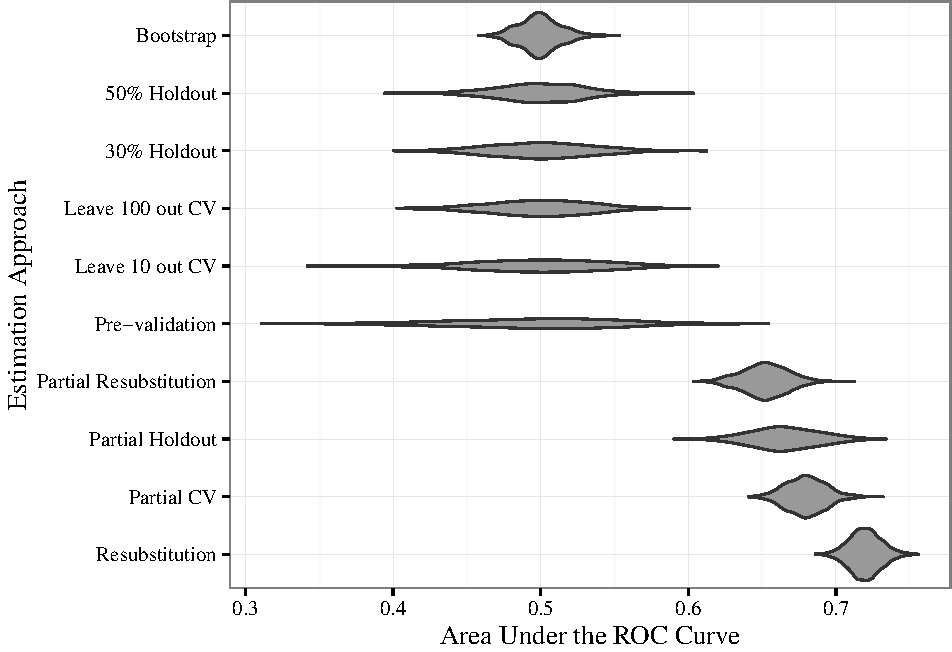
\includegraphics{paper_files/figure-latex/cvsims-1.pdf}
\caption{Comparison of different approaches to estimating the Area Under
the ROC Curve (AUC) in the setting where a dataset is used to both
develop the signature and evaluate its performance. The violin plots
show mirrored density estimates for the AUC for 1000 replicates of the
numerical experiment. In each replicate, there are 1000 observations and
500 features. The true value of the AUC is 0.5. CV = Cross validation.
\label{fig1}}
\end{figure}

\begin{figure}[htbp]
\centering
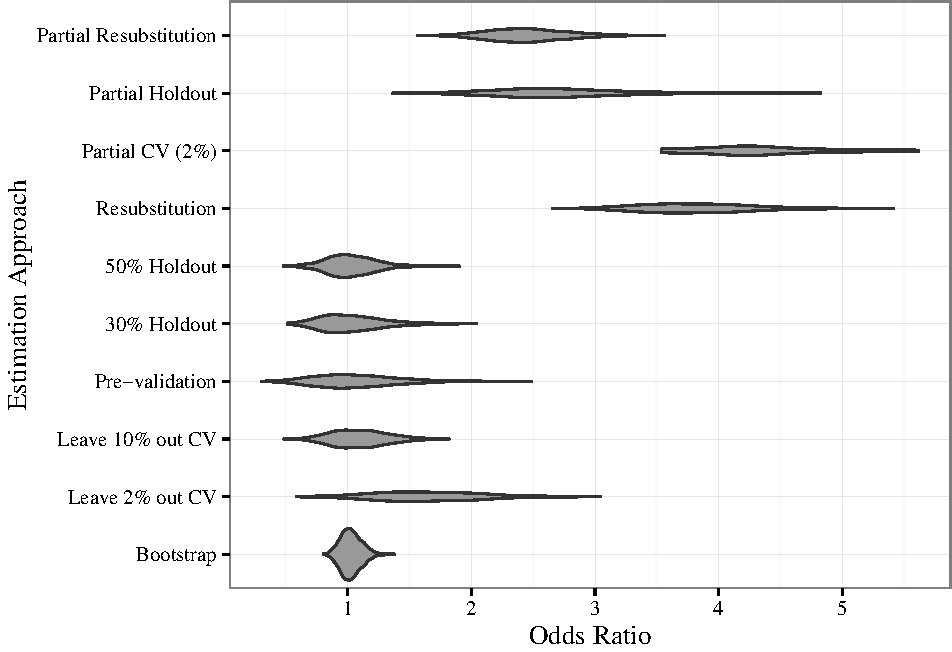
\includegraphics{paper_files/figure-latex/cvsims2-1.pdf}
\caption{Comparison of different approaches to estimating the odds ratio
(OR) in the setting where a dataset is used to both develop the
signature and evaluate its performance. The violin plots show mirrored
density estimates for the log OR for 1000 replicates of the numerical
experiment. In each replicate, there are 1000 observations and 500
features. The true value of the OR is 1.0. CV = Cross validation.
\label{fig2}}
\end{figure}

\begin{longtable}[c]{@{}lrrrrrr@{}}
\caption{Comparison of different approaches to estimating the Area Under
the ROC Curve (AUC) and the log odds ratio (OR) in the setting where a
dataset is used to both develop the signature and evaluate its
performance. The true value of the AUC is 0.5 and the true value of the
Log OR is 0.0. Estimates are based on 1000 replicates of the numerical
experiment. In each replicate, there are 1000 observations and 500
features. CV = Cross validation.}\tabularnewline
\toprule
Approach & mean AUC & std.dev AUC & Bias AUC & mean OR & std.dev OR &
Bias OR\tabularnewline
\midrule
\endfirsthead
\toprule
Approach & mean AUC & std.dev AUC & Bias AUC & mean OR & std.dev OR &
Bias OR\tabularnewline
\midrule
\endhead
Resubstitution & 0.72 & 0.01 & 0.22 & 1.33 & 0.12 & 1.33\tabularnewline
Partial CV & 0.68 & 0.01 & 0.18 & 1.02 & 0.12 & 1.02\tabularnewline
Partial Holdout & 0.67 & 0.02 & 0.17 & 0.97 & 0.19 & 0.97\tabularnewline
Partial Resubstitution & 0.65 & 0.02 & 0.15 & 0.88 & 0.12 &
0.88\tabularnewline
Pre-validation & 0.50 & 0.05 & 0.00 & -0.01 & 0.32 &
-0.01\tabularnewline
Leave 10 out CV & 0.50 & 0.04 & 0.00 & 0.00 & 0.25 & 0.00\tabularnewline
Leave 100 out CV & 0.50 & 0.03 & 0.00 & 0.00 & 0.20 &
0.00\tabularnewline
30\% Holdout & 0.50 & 0.03 & 0.00 & 0.00 & 0.24 & 0.00\tabularnewline
50\% Holdout & 0.50 & 0.03 & 0.00 & 0.00 & 0.20 & 0.00\tabularnewline
Bootstrap & 0.50 & 0.01 & 0.00 & 0.00 & 0.08 & 0.00\tabularnewline
\bottomrule
\end{longtable}

Not surprisingly, the resubstitution estimates are optimistically
biased: the naive resubstitution estimate of the AUC is 44\% larger than
it should be and the OR estimate is over 2 times higher than it should
be, on average. Partial resubstitution, partial holdout, and partial
cross-validation estimates do not ameliorate the bias very much.
Investigators often feel as though partial holdout estimates are close
to valid, as only half of the data are used to form the estimates,
however here we see that these versions are still severely biased and
should not be reported as valid assessments of the performance of
biomarker signatures.

All of the proposed remedies to avoid these biases are successful and
are unbiased, with their mean AUCs being nearly 0.5 and the mean ORs
being nearly 1. We can compare the spread of the distributions to get a
sense of the differences in precision of the estimates. The bootstrap
approach appears to be the most precise of the unbiased estimates,
followed by the cross-validation, holdout, and finally the
pre-validation. The bootstrap, as intended, is a more efficient,
smoothed version of the cross validation estimate (Figure \ref{fig1},
\ref{fig2}). It provides the best balance between allocating data to
precisely train the signature and having independent data remaining to
precisely estimate the statistic \(\phi\).

\subsection{Data Analysis}\label{data-analysis}

The signature development procedure was described in the introduction.
There is both a feature selection step, and a multivariable estimation
step. This results in a continuous signature which is the linear
predictor of a Cox regression model. The signature is dichotomized by
selecting the cutoff that yields the most significant log-rank statistic
for comparing the resulting risk groups. Discrimination of the signature
is assessed using the concordance statistic as implemented in the
\texttt{survival} package in \texttt{R} \citep{survival}. To paraphrase
the help file: this is defined as the probability of agreement for any
two randomly chosen observations, which in this case means that the
observation with the shorter survival time also has the larger signature
value. This is similar to an interpretation of the AUC for binary data.

First we fit the signature using the entire observation cohort (n = 62).
The signature was then evaluated on the same dataset. The survival plot
on the left side of Figure \ref{fig2} shows extreme separation between
the two risk groups (HR = 20, p \textless{} 0.001), consistent with the
reported JBL.10 signature, and the estimated concordance is 0.87. After
correctly accounting for the selection process, our estimates of
association and discrimination are much less impressive.

The right plot in Figure \ref{fig2} shows the survival curves for the
two risk groups using the pre-validated estimates of the risk score. We
partitioned the 62 observations into 8 groups of 6 and 2 groups of 7.
Then for each group \(b\), we fit the model using \(S_{-b}\) and
obtained prevalidated estimates for \(S_{b}\). The survival curves plot
the survival times for comparing risk groups using the prevalidated
estimates. The separation is much less impressive. The concordance
between the prevalidated signature and the survival times is 0.61,
indicating much worse discrimination.

\begin{figure}[htbp]
\centering
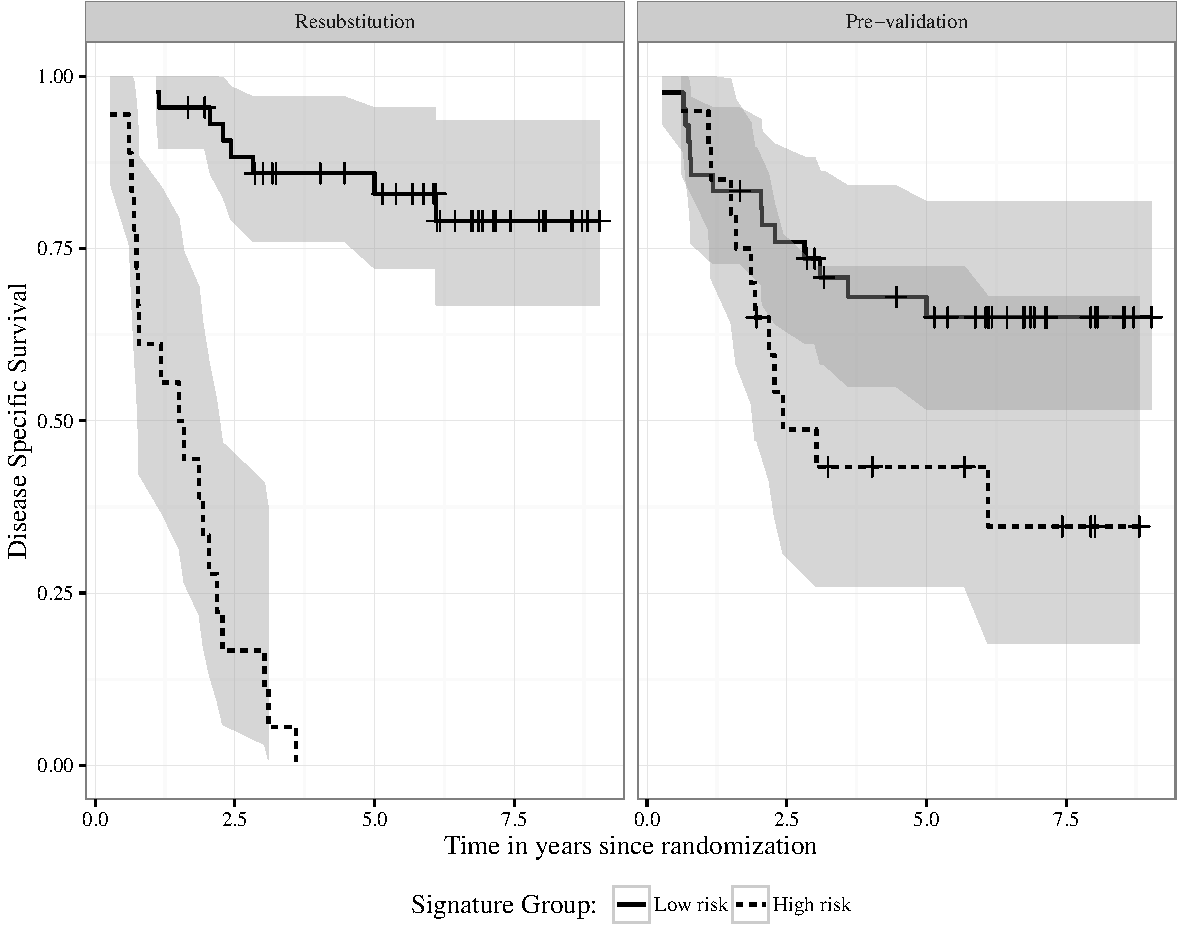
\includegraphics{paper_files/figure-latex/examppresub-1.pdf}
\caption{Comparison of survival by gene expression based risk signature.
The left plot shows the resubstitution estimate, while the right plot
shows the pre-validated estimate. \label{fig2}}
\end{figure}

\begin{figure}[htbp]
\centering
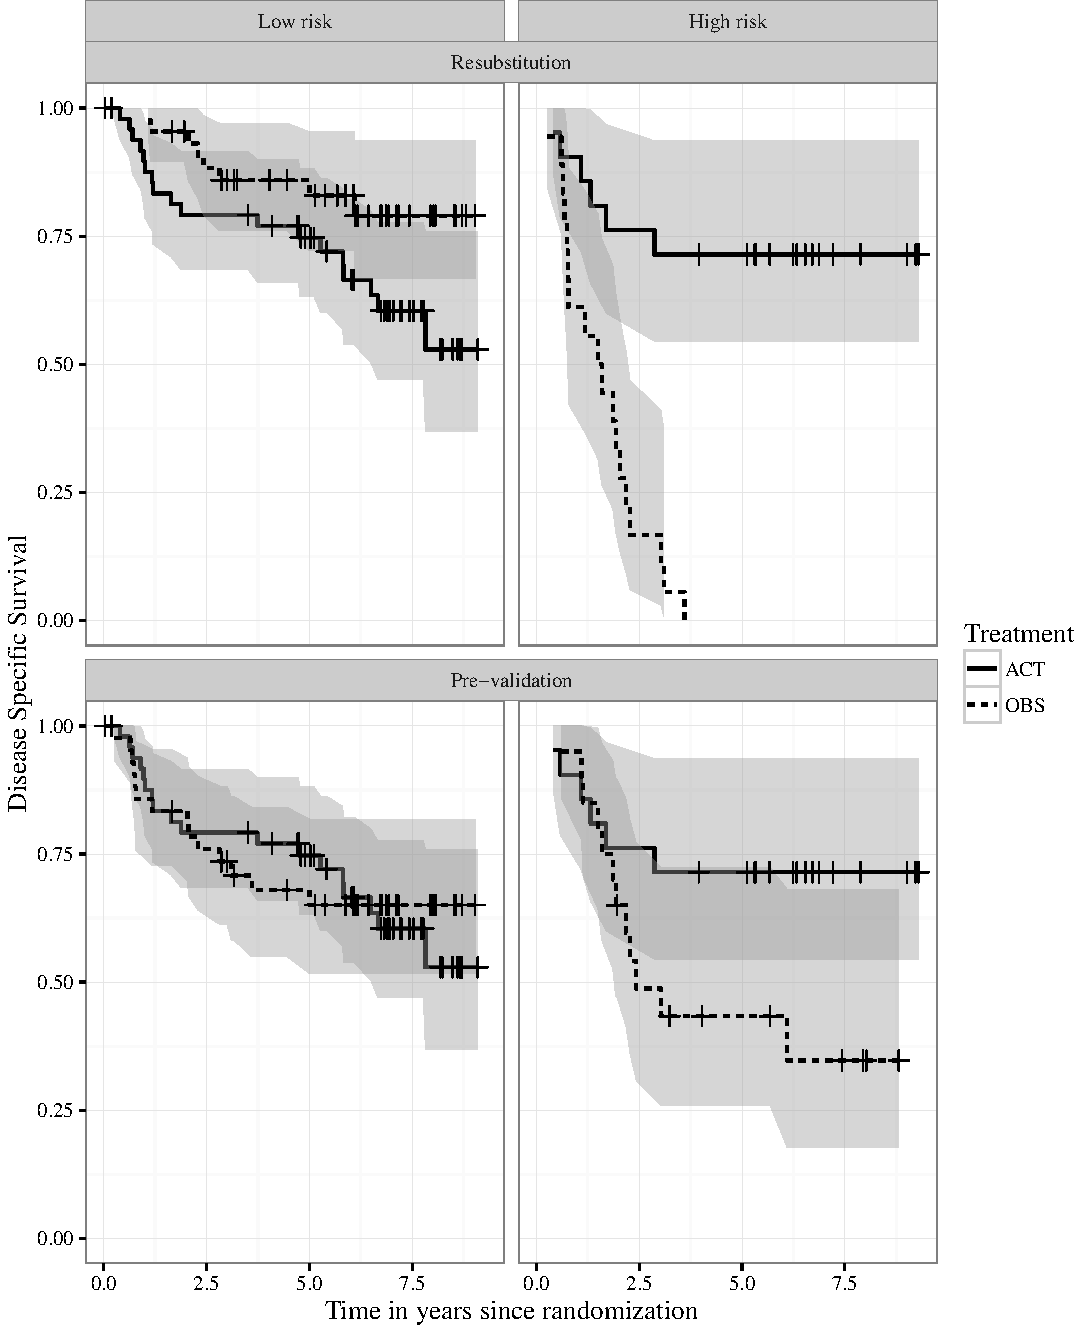
\includegraphics{paper_files/figure-latex/inter1-1.pdf}
\caption{Survival curves comparing the treatment effect by gene
expression signature risk group. The top set of plots shows the partial
resubstitution based signature and the bottom row shows the
pre-validated signature estimates. \label{fig3}}
\end{figure}

\begin{longtable}[c]{@{}lllll@{}}
\caption{Hazard ratios and 95\% confidence intervals from separate Cox
regression models that adjust for tumor histologic subtype, stages, age,
and sex. Rows labeled `High risk vs low risk' show the hazard ratio for
the signature-based risk group comparison. The rows labeled `Trt/Risk
interaction' show the hazard ratio for the interaction term of treatment
by signature-based risk group. The partial substitution estimates are
dramatically optimistically biased. \label{adjhr}}\tabularnewline
\toprule
Method & Comparison & Hazard Ratio & 95\% CI & Adjusted p\tabularnewline
\midrule
\endfirsthead
\toprule
Method & Comparison & Hazard Ratio & 95\% CI & Adjusted p\tabularnewline
\midrule
\endhead
\textbf{Partial Resubstitution} & High Risk vs Low Risk & 38.9 & 9.2 to
164.7 & \textless{} 0.001\tabularnewline
& Trt/Risk interaction & 14.7 & 3.2 to 67.0 & \textless{}
0.001\tabularnewline
\textbf{Prevalidation} & High Risk vs Low Risk & 1.9 & 0.8 to 4.3 &
0.122\tabularnewline
& Trt/Risk interaction & 1.8 & 0.5 to 6.5 & 0.395\tabularnewline
\bottomrule
\end{longtable}

We also show plots to assess the ability of the signature to be useful
for treatment selection (Figure \ref{fig3}). These plots show the
survival curves comparing treatment arms grouped in panels by the risk
score. As described by \citet{polley2013statistical}, the idea is to
determine whether the treatment is beneficial in one group and not
benficial or harmful in another group, indicating that different
treatment decisions would be made based on the signature. On one hand,
the overfit signature shows dramatic differences in treatment efficacy
between the low risk and high risk groups. In fact it appears that the
treatment is harmful in the low risk group, but highly beneficial in the
high risk group, a very rare finding. The prevalidated signature on the
other hand, shows differences that are much less dramatic. It appears
that the treatment is mildly beneficial in both groups, possibly to a
higher degree in the high risk group. This suggests that the dramatic
predictive value of the signature was merely an artifact of the
overfitting process on the OBS arm, as pointed out by
\citet{simon2011re}.

In a multivariable Cox model we observe similar trends when comparing
the prevalidated signature to the overfit signature. We fit two
regression models. In the first, the aim is to assess the prognostic
value of the signature by estimating the hazard ratio for the high risk
versus low risk groups, adjusted for tumor histologic subtype, stage,
age, and sex. In the second model, the idea is to assess the predictive
value of the signature by estimating the treatment by signature
interaction effect, adjusting for the same clinical covariates. The
results are reported in Table \ref{adjhr}. For the partial
resubstitution approach, we find an extreme hazard ratio of nearly 40
for the prognostic effect, and a strong and significant treatment by
signature interaction. Using the prevalidated signature, the effect
estimates are much smaller and insignificant in comparison to the
standard clinical features. Note that the inference from the
pre-validated model is not exactly correct either, because the procedure
induces a correlation among the observations. Despite this, these
results are unimpressive and would not be considered promising for
clinical use.

\subsection{Additional Examples}\label{additional-examples}

Examples of resubstitution estimates of performance are highly prevalent
in the literature. \citet{zhu2010prognostic} was not unique in that
sense, but rather they should be commended for their commitment to
making their data, methods, and analysis code publically available,
which allowed us to reproduce and reanalyze their study. More often, the
methods are obfuscated through vague and non-standard descriptions,
short methods sections, and hidden data analysis code. Most of the time,
a resubstitution analysis can be discovered only through a very careful
scrutiny of the methods and supplementary materials, if at all. Here we
give some additional examples.

\citet{van2002gene} used gene expression measurements to develop a
signature and predict clinical outcome of patients with axillary lymph
node-negative breast cancer (metastatic disease within 5 years versus
disease-free at 5 years). The signature was developed using a stepwise
selection and classification procedure, in which a subset of the genes
was first selected using all of the subjects, then further subsets were
selected using cross-validation until they arrived at a 70 gene
signature. This is the classic form of the partial cross-validation as
we've described above. The resubstitution estimate of the odds ratio to
develop distant metastasis within 5-years was estimated to be 28, with
\(p < 0.0001\). A later study of a similar population used similar gene
expression profiling approach, but with a valid split sample holdout
validation approach \citep{wang2005gene}. A univariate analysis of the
locked-down signature evaluated on the holdout set gave a much more
conservative odds ratio estimate of 5.7 for distant metastasis within 5
years.

\citet{zhang2001recursive} describe a tree-based partitioning approach
to use gene expression data to classify specimens as either cancer or
normal tissue. Again, from a large number of candidate genes, a subset
of three genes is identified using the entire set of 48 tissue
specimens. Then, the cutoff values for the classifications are
re-estimated using cross validation. This is yet again the classic form
of partial cross validation that we have shown to be biased, contrary to
their reports of ``unbiased'' estimates of 6-8\% missclassification
rates. This key detail of the analysis is only briefly described in the
results section.

\section{Discussion}\label{discussion}

All statistics, whether they assess calibration or discrimination or
something else, are subject to bias due to overfitting. Remedies to this
type of bias are well-studied in the statistical literature and here we
have demonstrated how they can be implemented in a real scenario. Sadly,
reports of strong associations with overfit biomarker signatures are all
too common in the medical literature. The amount of bias that is
possible is not known and can be difficult to decipher based on study
reports. It is imperative that investigators and journal editors take
overfitting bias seriously to ensure that signature estimates are valid.
Unfortunately this often results in study reports that are far less
optimistic than usual.

The \citet{zhu2010prognostic} paper used the approach of identifying a
signature using the control arm of the trial, evaluating it using the
combined control and treatment arms, and then hoping that the signature
would be useful for treatment selection. This approach has been shown to
be invalid \citep{simon2011re} for identifying a predictive signature,
and indeed we show that the resubstitution aspect of the evaluation
likely led to overstatments of the size of the signature effect.
Properly doing cross-validation for estimating the calibration of the
signature and doing pre-validation for assessment of the discrimination
of the signature show that the associations are much more modest.

When we assess the signature on the independent treatment arm, we see
that there is no significant difference between the risk groups. This
raises the question of whether it is appropriate to use non-random
splits of the dataset in order to obtain valid estimates of the
calibration or discrimination. Instead of treatment arms, we could
imagine a large multi-center study, and we could split the data into
disjoint subgroups based on the center. Specifically, suppose we split
the development dataset \(S\) into \(S_1\) and \(S_2\) according to a
discrete covariate \(X\) that takes on levels 1 or 2. The we develop a
signature \(f_{S_1}\) using \(S_1\) and evaluate it on \(S_2\) by
estimating \(\hat{E}[\phi_{f_{S_1}}(S_2)]\). This is an estimate not of
\(E_\mathcal{P}[\phi_f(S)]\), but rather
\(E_{\mathcal{P}_2}[\phi_f(S)]\), where \(\mathcal{P}_2\) is the
distribution for the sub-population with \(X = 2\) that \(S_2\) is a
sample from. This estimate would only be recommended if the signature is
intended for use in that specific subpopulation, and if that were the
case, then it doesn't make much sense to develop the signature using the
subpopulation \(\mathcal{P}_1\). If these groups differed substantially,
then we would not expect the signature to perform adequately. The
differences in performance may depend on many factors, including how
\(X\) is associated with the distribution of the features and the
outcome. If a signature becomes broadly used in clinics, these
center-to-center differences would be important to assess as a part of
signature efficacy surveillance.

\section{Note}\label{note}

All analysis code and the source files for this manuscript is available
from the authors' webpage.

\renewcommand\refname{References}
\bibliography{paper}

\end{document}
